\documentclass[sigconf,nonacm]{acmart}

\usepackage{booktabs}
\usepackage{listings}
\usepackage{xcolor}

\definecolor{pine}{HTML}{1C9970}
\definecolor{amber}{HTML}{C4761A}
\definecolor{cmt}{HTML}{6B7570}

\lstset{
  basicstyle=\ttfamily\scriptsize,
  commentstyle=\color{cmt}\itshape,
  keywordstyle=\color{pine}\bfseries,
  breaklines=true, columns=fullflexible,
  xleftmargin=6pt, framexleftmargin=3pt,
  frame=leftline, rulecolor=\color{pine!45},
  morecomment=[l]{\%\%},
  morekeywords={not},
  literate={<-}{{$\leftarrow$}}1,
}

\settopmatter{printacmref=false}
\renewcommand\footnotetextcopyrightpermission[1]{}

\begin{document}

\title{Approve Once: Relocating Human Oversight from Decisions to the Logic
that Produces Them}

\author{ACM Summer School on Responsible AI}
\affiliation{\institution{Group 3: Human-Centred, Agentic, Decision-Support AI}
  \country{}}

\begin{abstract}
Requirements for a ``human in the loop'' over consequential automated decisions
are widespread, but per-decision oversight scales linearly with volume and
degrades into rubber-stamping precisely where it matters most: where the
reviewer cannot independently verify the output under review. We describe and
implement an alternative. The decision logic is extracted from the model into an
inspectable database of universally quantified Horn clauses; an agent may
\emph{propose} rules and facts but never infers; and human approval attaches to
\emph{rules} rather than to decisions. Because a rule governs every future case
its body matches, oversight amortises: in a run over 1{,}000 real credit
applications, sixteen acts of review governed 589 decisions. We report three
further results. On a synthetic domain generated from a withheld rule set, the
rule miner recovers all three generating rules exactly and ranks them first,
alongside five plausible near-misses---giving, unusually, ground truth for
\emph{rules} rather than predictions. Encoding a written lending policy revealed
that the policy was silent on 11\% of cases, a gap its authors had not noticed
and which the system surfaced only because it refuses to guess. And a governance
invariant---that no critical decision may rest on an unapproved rule---is
enforced structurally and audited across every decision, with zero violations.
We are explicit about what we have \emph{not} shown: no human has yet reviewed a
rule in this system, and we describe the experiment that would settle it.
\end{abstract}

\keywords{meaningful human control, human oversight, neurosymbolic systems,
Datalog, explainability, agentic AI, EU AI Act Article 14}

\maketitle

\section{The problem with a human in the loop}

Regulatory and organisational responses to automated decision-making converge on
a common remedy: place a human in the loop. EU AI Act Article~14 requires that
high-risk systems be subject to effective human oversight. The difficulty is
that the remedy is usually operationalised \emph{per decision}---a reviewer
approves or rejects individual outputs---and per-decision oversight has two
structural problems.

First, it does not scale. Oversight cost is flat at one review per decision,
however large the caseload grows.

Second, and more seriously, it degrades into ceremony exactly where it is most
needed. Where the reviewer cannot independently verify the output---because the
model's reasoning is unavailable, or because verification would take longer than
the decision itself---a signature transfers accountability without improving the
decision. Green~\cite{green2022} argues that human-oversight requirements often
function as legitimacy theatre for this reason; the empirical literature on
automation bias and appropriate reliance points the same
way~\cite{parasuraman1997,bucinca2021,bansal2021}.

Our claim is that the failure is not of oversight but of \emph{unit}. Reviewing
a decision is work that must be repeated. Reviewing the \emph{logic} that
produces decisions is work that amortises.

\section{Design}

\subsection{The architectural commitment}

The system rests on one commitment: \textbf{the agent proposes; only the engine
infers.} A language model may draft candidate facts and candidate rules. It
never produces a decision. Inference is a terminating Datalog fixpoint over
function-free Horn clauses with stratified negation, so identical facts and
rules yield identical answers.

This is how determinism and explainability survive contact with a language
model. Nondeterminism is quarantined upstream of a human approval gate;
everything downstream is reproducible. A hallucinated predicate does not become
a bad decision---the vocabulary is closed and validation runs before the review
queue, so it becomes a discarded proposal that no reviewer ever sees.

The choice of Datalog over richer formalisms is deliberate. Prolog is
Turing-complete, so a recursive rule an agent adds can fail to terminate. Answer
Set Programming admits multiple answer sets, undercutting the determinism claim,
and its explanations must be reconstructed. Datalog is decidable and
terminating, and its proof tree \emph{is} the explanation.

\subsection{Rules carry their governance}

A rule is not merely a clause. It carries provenance, an approver, a usage
count, and an accuracy record:

\begin{lstlisting}
rule r0003 [p=0.80, origin=mined, status=approved,
            by="reviewer-jd", support=214, used=5,
            right="3/4"]
  high_risk(A) <- overdrawn(A), thin_savings(A).
\end{lstlisting}

Two fields carry most of the design's weight. The usage count is the
amortisation figure. The accuracy tally makes a rule's strength auditable rather
than asserted: a reviewer sees $p{=}0.80$ claimed against $3/4$ observed and can
judge the gap. Where the two diverge past a threshold, the rule returns for
re-review---the single exception to permanence, justified because the evidence
changed rather than because the reviewer is being asked to repeat themselves.

\subsection{Identity, and why approve-once needs it}

Rules are keyed by a \emph{canonical} hash: variables renumbered by first
appearance, body literals sorted. Under this key,
\lstinline|decline(A) <- overdrawn(A), thin_file(A)| and
\lstinline|decline(Z) <- thin_file(Z), overdrawn(Z)| are the same rule.

Without canonicalisation, ``approve once'' degrades silently. An agent
re-proposes settled logic in different syntax, a reviewer approves it again, and
the amortisation ratio collapses to one review per proposal while every
component appears to work. Identity is the primary key in the persistence layer,
so this is a constraint the database enforces rather than a convention the
application remembers.

\subsection{Criticality routes review; approval attaches to rules}

Criticality is a property of the \emph{query}; approval is a property of the
\emph{rule}. A rule proposed in a routine context becomes \textsc{provisional}
and is usable immediately, with offline review queued. A rule needed by a
critical query becomes \textsc{pending\_online} and \emph{blocks} that query.

The resulting invariant: \textbf{a critical decision can only ever be produced by
a derivation in which every rule is approved.} It is enforced by handing the
engine a filtered rule set, so an unapproved rule cannot contribute even
accidentally, and re-audited afterwards over the full query log.

The provisional lane is a deliberate risk: routine work proceeds on unreviewed
logic. The cost is made enumerable rather than hidden---rejecting a provisional
rule lists every decision that used it, across sessions.

\subsection{Missing information produces bounds, not guesses}

Facts are three-valued: \textsc{true}, \textsc{false}, \textsc{unknown}.
Absence is not falsity. Where facts are unknown, the system reports an interval
$[L,U]$ spanning every way they could resolve, computed by pinning unknowns to
their answer-minimising and answer-maximising values. For monotone programs this
requires two evaluations rather than $2^k$; only unknowns appearing in both
polarities are enumerated. The fast path is verified against exhaustive
enumeration on randomly generated programs including negation.

The width of the interval is the value of the missing information, which makes
the next action determinate rather than a matter of judgement:

\begin{lstlisting}
Answer: P = [0.00, 0.70]
Missing information, ranked by whether it
would change anything:
  app_gap has a guarantor   [DECISIVE]
      if true -> 0.00, if false -> 0.70
\end{lstlisting}

Unknowns that would change nothing are not offered. A system that asks for
information it will not use trains people to stop answering.

\subsection{Evidence follows provenance}

Rules arrive from three origins, and each asks the reviewer a different
question. A rule extracted from a written policy cites its clause: the question
is \emph{does this faithfully encode the clause?} A rule mined from labelled
cases carries support, precision, examples and counterexamples: the question is
\emph{is this correlation also a reason?} The review interface renders them
differently on purpose. Presented identically, a reviewer would answer the
easier question in both cases.

\subsection{One engine, two front ends}

The system is operated through a control room: a single page showing the rule
base, the cases still needing a person, an inspector that renders either a
rule's review evidence or a decision's proof, and the accountability record.
Screening runs in batches against the live engine, so the governance behaviour
is visible rather than described---starting a campaign before the rules are
approved produces blocked rows naming the rules each case is waiting on, and
those rows clear when the rules are approved.

We adopted this layout deliberately from our own earlier client-side prototype,
discussed in Section~\ref{sec:recruitment}, because the operational framing was
right even where what sat behind it was not. What changed is the referent: there
a fleet of a hundred simulated agents screened CVs and every screened CV became
a human review; here the fleet is the \emph{rule base}, a rule is reviewed once,
and the component that decides is the one that also writes the proof.

\section{Evaluation}

Three domain packs share the engine and no code: consumer credit over the UCI
Statlog German Credit data~\cite{hofmann1994} with a written lending policy, a
synthetic benefits-eligibility domain, and a recruitment campaign reproducing
the scenario of our own earlier prototype.

\subsection{Oversight amortises}

\begin{figure}[t]
  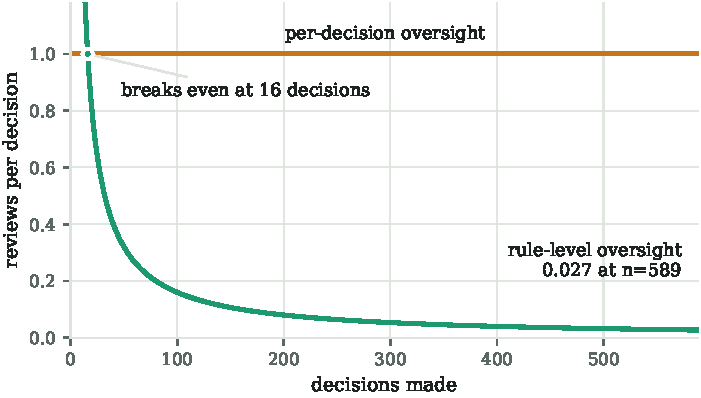
\includegraphics[width=\columnwidth]{figures/amortisation.pdf}
  \caption{Oversight cost per decision over a run of 1{,}000 credit
  applications. Per-decision oversight costs one review per decision by
  definition. Rule-level oversight is measured: cumulative approved rules over
  cumulative decisions. Reviews are paid up front, so the approach is initially
  more expensive and breaks even after 16 decisions; at $n{=}589$ the cost is
  $0.027$ reviews per decision, and still falling.}
  \label{fig:amort}
\end{figure}

Figure~\ref{fig:amort} shows the central result. Sixteen acts of review governed
589 decisions---36.8 decisions per review, with the ratio still improving as the
rule base matured. The approach is not free at the outset: reviews are paid
before any decision is made, so rule-level oversight is initially \emph{more}
expensive per decision and breaks even at 16. For a caseload of a few dozen it
would not be worth the machinery; the argument is about volume.

We report this figure with a caveat that cost us an earlier draft. An initial
version divided \emph{rule applications} by reviews and obtained 66.7. Several
rules fire per decision, so that ratio overstates the claim by exactly that
factor. Both are now reported separately; the decision-denominated figure is the
defensible one.

\subsection{The miner recovers the right rules}

\begin{figure}[t]
  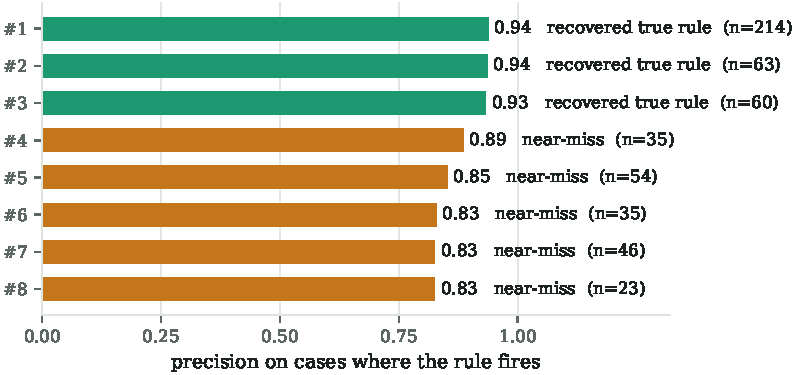
\includegraphics[width=\columnwidth]{figures/recovery.pdf}
  \caption{Mined proposals on the synthetic pack, ranked by precision. The three
  rules that generated the data are recovered exactly and rank first. Five
  plausible near-misses follow. Two attributes in the domain bear on nothing by
  construction; no proposal uses either.}
  \label{fig:recovery}
\end{figure}

The synthetic pack is generated from a rule set that is then withheld, which
permits a question real data cannot answer: not \emph{does this rule predict
well}, but \emph{is it the right rule}. Figure~\ref{fig:recovery} shows all
three generating rules recovered exactly and ranked first among eight proposals.

The five near-misses are the interesting part, because two are wrong in ways a
reviewer can check against written policy. One grants eligibility on a recent
award, which policy clause s4.1 says should trigger \emph{referral}. Another
reproduces the disability route with the capital-limit guard silently dropped,
and would pay applicants holding savings above the limit. Both sit at 83--85\%
precision and look entirely respectable. This is the concrete case for a human
reading rules rather than trusting a threshold.

Reaching this result required a correction worth recording. An initial miner
searched only positive conjunctions and therefore could not express
\lstinline|not savings_over_limit|. Rather than failing visibly, it
\emph{approximated} the rule with whatever correlated---including the two noise
attributes---recovering one rule of three. Admitting negated literals took
recovery to three of three and eliminated the noise proposals. A miner that
cannot say ``not'' does not merely miss rules; it produces rules that are wrong
in a way the evidence cannot reveal.

\subsection{The system found a gap in the written policy}

We authored a lending policy, extracted it into eight cited rules, and observed
that the system then declined to decide 11\% of cases. Clause s7.1 covers
elevated risk \emph{without} mitigating security; s7.2 covers security
\emph{without} elevated risk; neither covers an applicant with both. We had not
noticed.

This is the practical payoff of distinguishing ``no applicable logic'' from
``no''. A scoring model would have produced a confident number for every one of
those applicants. Competing outcomes are deliberately never normalised: if all
are low, the rule base has nothing to say, and normalising near-zero values
would disguise ignorance as a confident split.

\subsection{The same campaign, against our own earlier prototype}
\label{sec:recruitment}

Before building the rule base we had built a conventional agentic prototype for
the same brief: a hundred simulated screening agents over an 8{,}000-applicant,
1{,}000-hire recruitment campaign, each agent able to reject a CV on a confirmed
mismatch or flag it for a person. It is a useful baseline precisely because we
wrote it, and because running it exposes two things its interface does not say.

First, it does not reduce human work. Of 8{,}000 CVs it flags 5{,}621 for review
(70\%), of which 4{,}012 are cases where the requirements were \emph{met} and a
person must still decide, plus 237 sampled rejection audits: 5{,}858 human
reviews to make 1{,}000 hires, or 5.9 reviews per hire. Second, its interface
states of agent rejections that ``each can be reopened'', yet 2{,}142 of 2{,}379
rejections (90\%) are never surfaced to any human, and the screening logic is a
hard-coded function that cannot be inspected or approved at all.

We rebuilt the scenario as a third domain pack, with the screening policy written
as prose and extracted into eight cited rules. Table~\ref{tab:recruitment}
compares the two on the identical campaign.

\begin{table}[t]
  \caption{The same 8{,}000-applicant campaign under both systems.}
  \label{tab:recruitment}
  \begin{tabular}{lrr}
    \toprule
    & \textbf{Agent fleet} & \textbf{Rule base} \\
    \midrule
    One-off rule reviews        & ---     & 8 \\
    Human case reviews          & 5{,}858 & 2{,}558 \\
    Decided without a person    & 0       & 5{,}442 \\
    Screening logic inspectable & no      & yes \\
    Wrong rejections measurable & no      & yes \\
    \bottomrule
  \end{tabular}
\end{table}

The last row matters more than the counts. In the agent fleet a rejection is
correct by construction: it fires only on an explicit unmet requirement, and
there is no notion of a suitable applicant wrongly rejected, so an auditor has
nothing to find and contestability can be offered but never exercised. The
recruitment pack carries a withheld suitability label, and against it
\textbf{26.4\% of automatic rejections are of genuinely suitable applicants}.
That is not a good number. It is, however, a number---and the audit queue now
has something to find.

The pack also records two protected attributes that are deliberately \emph{not}
declared predicates, so no rule can be written or mined over either. Normalising
by band size, applicants over 40 are auto-rejected \emph{less} often than
younger ones (28\% against 38--39\%), because a timeline-conflict signal that
correlates with age routes them to human review instead. A disparity that runs
toward more human review is still a disparity, and it is visible only because
the attribute is recorded while being unavailable to the logic.

\subsection{Governance guarantees hold}

Across every critical decision in the credit run, the invariant audit reports
zero violations. The property is also checked directly: the test suite
constructs a state in which an approved rule is retroactively downgraded and
confirms the audit detects it, so the check is capable of failing.

\begin{table}[t]
  \caption{Measured results. All figures are produced by scripts in the
  repository; the two figures are generated from live runs rather than
  transcribed.}
  \label{tab:results}
  \begin{tabular}{lr}
    \toprule
    \textbf{Result} & \textbf{Value} \\
    \midrule
    Decisions per act of review & 36.8 \\
    Generating rules recovered exactly & 3 / 3 \\
    Proposals resting on noise attributes & 0 / 8 \\
    Cases on which written policy was silent & 11\% \\
    Governance invariant violations & 0 \\
    \bottomrule
  \end{tabular}
\end{table}

\section{Design principles}

Each of the following was earned by a defect we shipped and then fixed, not
derived from first principles.

\begin{enumerate}
\item \textbf{Put oversight where it amortises.} If oversight cost per decision
  is flat, the unit is wrong.
\item \textbf{Absence is not denial.} ``No applicable logic'' and ``no'' are
  different answers and must read differently.
\item \textbf{Unknowns must survive negation.} A fact blocked by a
  missing input is itself unknown. We shipped this wrong twice: a negated
  condition succeeded because nobody had recorded the fact underneath it, and an
  applicant was declined on an assumption no one had made.
\item \textbf{Approve the logic, not the text.} Identity must be invariant under
  renaming and reordering, or approve-once means nothing.
\item \textbf{Evidence follows provenance.} Different origins pose different
  questions and need different evidence.
\item \textbf{Make guarantees structural, not procedural.} Our lending policy
  forbids decisions resting on sex. That clause is deliberately \emph{not} a
  rule---a rule can state a condition but not the absence of a hidden
  correlation. Instead the attribute is absent from the vocabulary, so no rule
  can be written or mined over it. Review cannot reliably detect a proxy and
  should not be asked to.
\item \textbf{State the assumption in the output.} Combining independent
  supports by noisy-OR is a modelling commitment and frequently a wrong one; it
  appears in every explanation rather than inside the arithmetic.
\item \textbf{A system that cannot be wrong cannot be audited.} Screening
  logic whose rejections are correct by construction offers contestability as an
  affordance and can never exercise it. Build the ground truth that lets a
  decision be wrong, or the review queue is decoration.
\item \textbf{The price of speed must be enumerable.} Provisional rules keep
  routine work moving; rejecting one names every decision it touched.
\end{enumerate}

\section{Limitations}

\textbf{No human has reviewed a rule in this system.} The amortisation figure is
arithmetic over a working prototype, not evidence that reviewers review rules
well. If they cannot, the argument fails, and nothing in the present work would
detect it.

The experiment that would settle it is unusually clean, because the synthetic
pack supplies ground truth for \emph{rules}: reviewers are shown the eight
proposals of Figure~\ref{fig:recovery}, and the measurement is whether they
approve the correct three and reject the five near-misses, at what time cost,
and whether showing support and precision changes their accuracy. We regard this
as the necessary next step rather than future work.

\textbf{Credit assignment is crude.} Outcome feedback marks every rule in a
derivation right or wrong together, so a determination rule is blamed for
failures caused by its premises. Proper attribution requires something like a
Shapley value over the derivation.

\textbf{Rejection flags but does not reverse.} The system enumerates the
decisions a withdrawn rule touched and stops. Whether that invalidates them is a
judgement it should not make alone.

\textbf{The recruitment comparison is not like-for-like in every respect.}
The two systems partition work differently, and the baseline is our own
prototype rather than a deployed product. What the comparison establishes is
narrower than a benchmark and still worth stating: on identical inputs, moving
review from cases to rules cut human case reviews by 56\% while making the
screening logic inspectable and its error rate measurable for the first time.

\textbf{Accuracy figures on the credit pack are not a benchmark.} They score an
invented lending policy against real outcome data. The system detecting that its
own policy is poorly fitted is the machinery working, not a capability claim.

\section{Related work and positioning}

The inference engine is deliberately unoriginal. Datalog is well
understood~\cite{ceri1989}, and that is precisely why the determinism claim
holds. The contribution is not the engine but the governance layer over it:
canonical approve-once identity, criticality-routed review, enforced
approval-before-critical-use, and retroactive impact analysis.

Classical expert systems foundered partly on knowledge
acquisition~\cite{feigenbaum1980}. A language model that drafts candidate rules
under structured review is a different answer to that bottleneck than a
knowledge engineer with a notepad---and, critically, one whose output is
governed rather than trusted. Relative to work on appropriate
reliance~\cite{bucinca2021,bansal2021}, which studies how humans respond to
per-decision advice, we change the object of review rather than its presentation.

\section{Conclusion}

Moving human oversight from decisions to the logic that produces them makes
oversight amortise, makes decisions explainable by construction rather than by
narration, and makes it possible to guarantee structurally that a consequential
decision never rests on logic nobody approved. The prototype demonstrates that
these properties are jointly achievable. Whether humans review rules well enough
to realise the benefit is the open question, and it is answerable.

\begin{thebibliography}{9}
\bibitem{green2022} Ben Green. 2022. The Flaws of Policies Requiring Human
  Oversight of Government Algorithms. \emph{Computer Law \& Security Review} 45.
\bibitem{parasuraman1997} Raja Parasuraman and Victor Riley. 1997. Humans and
  Automation: Use, Misuse, Disuse, Abuse. \emph{Human Factors} 39, 2.
\bibitem{bucinca2021} Zana Bu\c{c}inca, Maja Barbara Malaya, and Krzysztof Z.
  Gajos. 2021. To Trust or to Think: Cognitive Forcing Functions Can Reduce
  Overreliance on AI in AI-assisted Decision-making. \emph{Proc. ACM HCI} 5.
\bibitem{bansal2021} Gagan Bansal et al. 2021. Does the Whole Exceed its Parts?
  The Effect of AI Explanations on Complementary Team Performance. \emph{CHI}.
\bibitem{ceri1989} Stefano Ceri, Georg Gottlob, and Letizia Tanca. 1989. What
  You Always Wanted to Know About Datalog. \emph{IEEE TKDE} 1, 1.
\bibitem{feigenbaum1980} Edward A. Feigenbaum. 1980. Knowledge Engineering: The
  Applied Side of Artificial Intelligence. Stanford University.
\bibitem{hofmann1994} Hans Hofmann. 1994. Statlog (German Credit Data). UCI
  Machine Learning Repository.
\end{thebibliography}

\end{document}
